%! Author = melek
%! Date = 9.06.2022

% Preamble
\documentclass[11pt]{article}

% Packages
\usepackage{amsmath}
\DeclareMathOperator*{\argmax}{argmax}

\usepackage{graphicx}
\usepackage{amssymb}
\usepackage{bm}

\graphicspath{ {../images/} }


% Document
\begin{document}

    \maketitle
    \setcounter{section}{10}


    \section{Exercises}

    \subsection{Question}

    Convert the equation of n-step o↵-policy TD (7.9) to semi-gradient form.
    Give accompanying definitions of the return for both the episodic and continuing cases.

    \subsection*{Answer}

    The answer is straight forward.
    We just need to take 7.9 as basis and modify it by using 11.6 after replacing $\hat{q}$ functions with $\hat{v}$ functions.
    Also note that importance sampling starts from t in n-step case.

    \noindent $ w_{t+n} = w_{t+n-1} + \alpha \rho_{t:t+n-1} [G_{t:t+n} - \hat{v}(S_t, w_{t+n-1}) ] \Delta\hat{v}(S_t, w_{t+n-1})$

    \hfill \break
    Episodic return:

    \noindent $ G_{t:t+n} = R_{t+1} + \ldots + \gamma^{n-1} R_{t+n} + \gamma^n \hat{v}(S_t,w_{t+n-1}) $

    \hfill \break
    \noindent Continuing return:

    \noindent $ G_{t:t+n} = R_{t+1} - \bar{R}_t + \ldots + R_{t+n} - \bar{R}_{t+n-1} + \hat{v}(S_t,w_{t+n-1}) $


    \subsection{Question}

    Convert the equations of n-step $Q( \sigma )$ (7.11 and 7.17) to semi-gradient form.
    Give definitions that cover both the episodic and continuing cases.

    \subsection*{Answer}

    Converted 7.11:

    \noindent $ w_{t+n} = w_{t+n-1} + \alpha \rho_{t+1:t+n} [G_{t:t+n} - \hat{q}(S_t,A_t, w_{t+n-1}) ] \Delta\hat{Q}(S_t,A_t, w_{t+n-1})$

    \hfill \break
    \noindent Converted 7.17:

    \noindent Episodic return.
    Note the last part is inspired by how average state value part in 7.7 is converted in 11.6 :

    \noindent $ G_{t:t+n} = R_{t+1} + \gamma  (\sigma_{t+1} \rho_{t+1} + (1-\sigma_{t+1}) \pi(A_{t+1}|S_{t+1})  ) (G_{t+1:t+n} - \hat{q}_{t+n-1}(S_{t+1},A_{t+1}, w_{t+n-1})) + \gamma^n \hat{q}(S_{t+n},A_{t+n}, w_{t+n-1}) $

    \hfill \break
    \noindent Continuing return.
    Note that conversion is done by applying the guidelines given slightly after 10.9.
    "We simply remove all s and replace all rewards by the difference between the reward and the true average reward":

    \noindent $ G_{t:t+n} = R_{t+1} - \bar{R_{t}} + (\sigma_{t+1} \rho_{t+1} + (1-\sigma_{t+1}) \pi(A_{t+1}|S_{t+1})  ) (G_{t+1:t+n} - \hat{q}_{t+n-1}(S_{t+1},A_{t+1}, w_{t+n-1})) + \hat{q}(S_{t+n},A_{t+n}, w_{t+n-1}) $


    \subsection{Question}

    (programming) Apply one-step semi-gradient Q-learning to Baird’s counterexample and show empirically that its weights diverge.

    \subsection*{Answer}

    Q-learning results actually found to converge.
    This may be due to a subtle error in my implementation.

    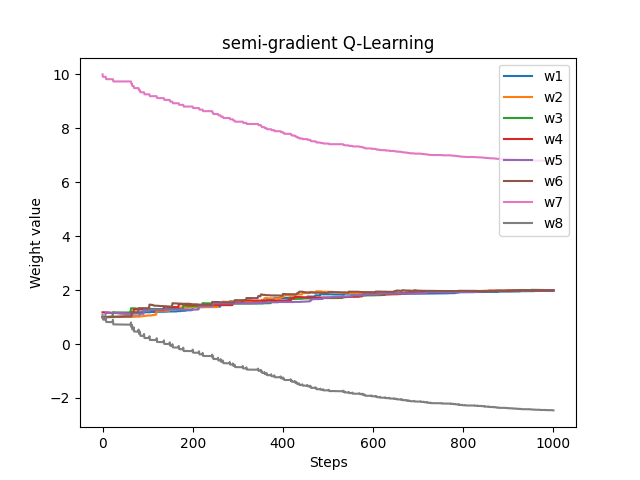
\includegraphics[scale=0.7]{exercise_11_3}

    \subsection{Question}

    Prove (11.24).
    Hint: Write the RE as an expectation over possible states s of the expectation of the squared error given that S t = s.
    Then add and subtract the true value of state s from the error (before squaring), grouping the subtracted true value with the return and the added true value with the estimated value.
    Then, if you expand the square, the most complex term will end up being zero, leaving you with (11.24).

    \subsection*{Answer}

    \noindent $ \bar{VE}(w) = \sum_{s \in S  } \mu(s) [v_\pi(s) - \hat{v}(s,w)]^2 = E [(v_\pi(s) - \hat{v}(s,w))^2] $   9.1

    \noindent $ \bar{RE}(w) = E [(G_t - \hat{v}(S_t,w))^2] $

    Hint is followed:

    \noindent $ \bar{RE}(w) = \sum_{s \in S  } \mu(s) [G_t(s) - \hat{v}(s,w)]^2 $

    \noindent $ \bar{RE}(w) = \sum_{s \in S  } \mu(s) [(G_t(s) - v_\pi(s)) + (v_\pi(s)  - \hat{v}(s,w))]^2 $

    \noindent $ \bar{RE}(w) = \sum_{s \in S  } \mu(s) [(G_t(s) - v_\pi(s))^2 + (v_\pi(s)  - \hat{v}(s,w))^2 + 2 (G_t(s) - v_\pi(s)) (v_\pi(s)  - \hat{v}(s,w))] $

    \noindent $ \bar{RE}(w) = E [(G_t(s) - v_\pi(s))^2] + E[ (v_\pi(s)  - \hat{v}(s,w))^2] +  E [2 (G_t(s) - v_\pi(s)) (v_\pi(s)  - \hat{v}(s,w))] $

    \noindent $ \bar{RE}(w) = E [(G_t(s) - v_\pi(s))^2] + \bar{VE}(w) +  E [2 (G_t(s) - v_\pi(s)) (v_\pi(s)  - \hat{v}(s,w))] $
    \hfill \break

    The hint says the most complex term will end up being zero.
    It is possibly because $ E[G_t] = E[v_\pi(s)] $.
    This would make the left most term end up being zero.
    However, for me, it is not clear, if this is the case, why we do not apply the same logic to the first expectation.

    Anyway, when the last term is zeroed out we are left with 11.24.

\end{document}


